%% FileName: jsai2016.tex
%% -*- coding: utf-8 -*-
%% Author: Shin Asakawa <asakawa@ieee.org>
%% CreationData: 20/Mar/2016
%%
%% This is a copyprotected file.
%% I, Shin Asakawa, have all the rights reserved.


%% definition of techinical terms
\newcommand{\AI}{{AI}}
\newcommand{\BP}{誤差逆伝播法}
\newcommand{\dropout}{dropout}
\newcommand{\GRU}{{GRU}}
\newcommand{\LSTM}{{LSTM}}
\newcommand{\ReLU}{整流線形ユニット}
\newcommand{\RNN}{リカレントニューラルネットワーク}
\newcommand{\RCNN}{領域畳込みニューラルネットワーク}
\newcommand{\sigmoid}{sigmoid}
\newcommand{\TANH}{$\tanh$}
\newcommand{\NN}{ニューラルネットワーク}


%% > まだコード書く段階でデータが見えていないのですが,訓練データ,検証デー
%% > タ,テストデータの3つにできるくらいデータ量はありますでしょうか。
%% https://www.reddit.com/r/MachineLearning/
%% https://www.reddit.com/r/MLQuestions/
%% https://www.reddit.com/r/mlclass/
%% から集めて,1703セットのQA が今アップされています。
%% できればもっと欲しいのですが,過去ログ等ご存知であればお教えください。

%% 過去ログがダメそうなら,stackoverflow の machine-learning タグ
%% http://stackoverflow.com/questions/tagged/machine-learning
%% を漁ろうかと思ってはいますが, html 構造の違い等が影響を与えないかが少し気にかかります。

\documentclass[twocolumn]{jarticle}

\usepackage{jsaiac}
\usepackage[dvipdfmx]{graphicx}
\usepackage{color}
\usepackage{url}

%%
\title{
%\jtitle{\LSTM を用いた質疑応答文の構築\\ ---Reddit/r/MLQuestions を用いて---}
%\etitle{Toward a Q--A system via {LSTM} for {R}eddit/r/{MLQ}uestions}
\jtitle{{LSTM}を用いた質疑応答システムによる\\人工知能知識習得の可能性の評価}
\etitle{An Evaluation of {Q}-{A} systems for Acquiring Knowledge of Artifitial Intelligence via {LSTM}}
}
%%英文は以下を使用
%\title{Style file for manuscripts of JSAI 20XX}

\jaddress{浅川伸一,東京女子大学,167--8585 東京都杉並区善福寺2--6--1, 03--5382--6746, asakawa@ieee.org.\\亀田 雅之,  m.kamedax@gmail.com}

\author{%
\jname{根岸 儀和\first{}}
\ename{Yoshikazu Negishi}
\and
\jname{小田 徳光\first{}}
\ename{Norimitsu Oda}
\and
\jname{岩井 健二}
\ename{Kenji Iwai}
\and
\jname{中村 彰宏}
\ename{Akihiro Nakamura}
\and
\jname{亀田 雅之}
\ename{Masayuki Kameda}
\and
\jname{浅川 伸一\second{}}
\ename{Shin Asakawa}
}

\affiliate{
  \jname{\first{}株式会社ロボケン}
  \ename{{R}obo{K}en {Co.} {L}td.}
  \and
  %% \jname{\fifth{}}
  %% \ename{{}}
  %% \and
  %% \jname{\third{}}
  %% \ename{{}}
  %% \and
  %% \jname{\fourth{}}
  %% \ename{{}}
  %% \and
\jname{\second{}東京女子大学}
\ename{Tokyo Woman's Christian University}
}



\graphicspath{{fig/}}  %% the directry cotaining the image files
\usepackage{float}     %% 図表をその場所に表示させる [H]オプション使用

\usepackage{atbegshi}
\AtBeginShipoutFirst{\special{pdf:tounicode EUC-UCS2}}
%% \usepackage[none]{hyphenat} %%% inhibit hyphenation

\usepackage{asamath}   %% Asakawa's math definition file
\DeclareRelationFont{JY1}{mc}{it}{}{OT1}{cmr}{it}{}
\DeclareRelationFont{JT1}{mc}{it}{}{OT1}{cmr}{it}{}
\DeclareFontShape{JY1}{mc}{m}{it}{<5> <6> <7> <8> <9> <10> sgen*min
    <10.95><12><14.4><17.28><20.74><24.88> min10
    <-> min10}{}
\DeclareFontShape{JT1}{mc}{m}{it}{<5> <6> <7> <8> <9> <10> sgen*tmin
    <10.95><12><14.4><17.28><20.74><24.88> tmin10
    <-> tmin10}{}
\DeclareRelationFont{JY1}{mc}{sl}{}{OT1}{cmr}{sl}{}
\DeclareRelationFont{JT1}{mc}{sl}{}{OT1}{cmr}{sl}{}
\DeclareFontShape{JY1}{mc}{m}{sl}{<5> <6> <7> <8> <9> <10> sgen*min
    <10.95><12><14.4><17.28><20.74><24.88> min10
    <-> min10}{}
\DeclareFontShape{JT1}{mc}{m}{sl}{<5> <6> <7> <8> <9> <10> sgen*tmin
    <10.95><12><14.4><17.28><20.74><24.88> tmin10
    <-> tmin10}{}
\DeclareRelationFont{JY1}{mc}{sc}{}{OT1}{cmr}{sc}{}
\DeclareRelationFont{JT1}{mc}{sc}{}{OT1}{cmr}{sc}{}
\DeclareFontShape{JY1}{mc}{m}{sc}{<5> <6> <7> <8> <9> <10> sgen*min
    <10.95><12><14.4><17.28><20.74><24.88> min10
    <-> min10}{}
\DeclareFontShape{JT1}{mc}{m}{sc}{<5> <6> <7> <8> <9> <10> sgen*tmin
    <10.95><12><14.4><17.28><20.74><24.88> tmin10
    <-> tmin10}{}
\DeclareRelationFont{JY1}{gt}{it}{}{OT1}{cmbx}{it}{}
\DeclareRelationFont{JT1}{gt}{it}{}{OT1}{cmbx}{it}{}
\DeclareFontShape{JY1}{mc}{bx}{it}{<5> <6> <7> <8> <9> <10> sgen*goth
    <10.95><12><14.4><17.28><20.74><24.88> goth10
    <-> goth10}{}
\DeclareFontShape{JT1}{mc}{bx}{it}{<5> <6> <7> <8> <9> <10> sgen*tgoth
    <10.95><12><14.4><17.28><20.74><24.88> tgoth10
    <-> tgoth10}{}
\DeclareRelationFont{JY1}{gt}{sl}{}{OT1}{cmbx}{sl}{}
\DeclareRelationFont{JT1}{gt}{sl}{}{OT1}{cmbx}{sl}{}
\DeclareFontShape{JY1}{mc}{bx}{sl}{<5> <6> <7> <8> <9> <10> sgen*goth
    <10.95><12><14.4><17.28><20.74><24.88> goth10
    <-> goth10}{}
\DeclareFontShape{JT1}{mc}{bx}{sl}{<5> <6> <7> <8> <9> <10> sgen*tgoth
    <10.95><12><14.4><17.28><20.74><24.88> tgoth10
    <-> tgoth10}{}
\DeclareRelationFont{JY1}{gt}{sc}{}{OT1}{cmbx}{sc}{}
\DeclareRelationFont{JT1}{gt}{sc}{}{OT1}{cmbx}{sc}{}
\DeclareFontShape{JY1}{mc}{bx}{sc}{<5> <6> <7> <8> <9> <10> sgen*goth
    <10.95><12><14.4><17.28><20.74><24.88> goth10
    <-> goth10}{}
\DeclareFontShape{JT1}{mc}{bx}{sc}{<5> <6> <7> <8> <9> <10> sgen*tgoth
    <10.95><12><14.4><17.28><20.74><24.88> tgoth10
    <-> tgoth10}{}
\DeclareRelationFont{JY1}{gt}{it}{}{OT1}{cmr}{it}{}
\DeclareRelationFont{JT1}{gt}{it}{}{OT1}{cmr}{it}{}
\DeclareFontShape{JY1}{gt}{m}{it}{<5> <6> <7> <8> <9> <10> sgen*goth
    <10.95><12><14.4><17.28><20.74><24.88> goth10
    <-> goth10}{}
\DeclareFontShape{JT1}{gt}{m}{it}{<5> <6> <7> <8> <9> <10> sgen*tgoth
    <10.95><12><14.4><17.28><20.74><24.88> tgoth10
    <-> tgoth10}{}
\endinput
%%%% end of jdummy.def     %% avoid warning while compiling .tex file with platex


%%
%\Vol{28}        %% <-- 28th(変更しないでください)
%\session{1I5-4}%% <-- 講演ID(必須)

\begin{abstract} %% 150 words maximun
We investigated two question-and-answer (Q-A) processing systems via LSTM.
A Sequence-2-Sequence model was compared to a vanilla LSTM to process the
machine learning thread in a reddit.com.  Based on our findings, we
proposed several possibilities to deal with this problem.  We discussed
further requirements to process Q-A specific problems that remain unsolved.
Suggestions might be obtained on sequential information processings,
combined with our results and requirements.
\end{abstract}

%\setcounter{page}{1}
\def\Style{``jsaiac.sty''}
\def\BibTeX{{\rm B\kern-.05em{\sc i\kern-.025em b}\kern-.08em%
 T\kern-.1667em\lower.7ex\hbox{E}\kern-.125emX}}
\def\JBibTeX{\leavevmode\lower .6ex\hbox{J}\kern-0.15em\BibTeX}
\def\LaTeXe{\LaTeX\kern.15em2$_{\textstyle\varepsilon}$}

\begin{document}
\maketitle

\section{はじめに}
%% 近年,猫画像のクラスタリング[1],
囲碁での人間への勝利~\cite{2016AlphaGo}等,人工知能技術が衆目を集め 関連す
る技術,知識に関する教育の需要が高まっている。しかし,人工知能の実装には統
計や機械学習の知識が必要であり,需要に対して十分な技術を持った技術者が不足
している状態である。%%と言える。
%%
%% そこで
我々は,「\AI を教える\AI」を作ることによってこの問題の解決ができないかを検
討した。現在,機械による学習を行う方法として,さまざまな e-learningシステム
が利用されている。しかし,それらのシステムは学習内容の提示と演習問題の組み
合わせからなっており,学習者に応じた適応的な教示ができるわけではない。現在
の人間の講師の利点は,学習者の理解の度合いや,欠落している知識などの学習状
態を推測し,学習の順序や演習問題の形式を適応的に変化させられる点とであると
言える。この適応性を実現する上では,学習の過程で学習者「AIを教えるAI」が頻
繁にやり取りを行う質疑応答による学習,いわば人間の教師における個人指導のよ
うなシステムであることが望ましいと考えられる。

人工知能による質疑応答には
\cite{2013Kalchbrenner_EMNLP,2015Wen_EMNLP,2015Lowe,2015Vinyals_NeuralConversationalModel,2015Shang,2015Soroni}
といった事例が挙げられる。
%% が,
学習という目的から,事前に質疑応答を選択肢やパターンとして限定することは難
しい。そのため,学習者が任意の表現で質問可能な自然言語による質疑応答システ
ムが望ましいといえる。そこで我々は,事前に特徴量の選択を必要としない,\NN
による自然言語処理を考え,一系列データを扱うことのできる\NN である
\LSTM(Long short-term memory, 図\ref{fig:LSTM})~\cite{1997LSTM}を用いたシス
テムの構築を想定した。%% 先述のように,学習を目的とした人工知能には,学習状
%% 態に合わせた適応が必要となる。しかし,\LSTM を用いた自動翻
%% 訳~\cite{2014Sutskever_Sequence_to_Sequence,2014Bahdanau_NMT}や画像への
%% ラベル付
%% け~\cite{2014Vinyals_Bengio_Show_and_Tell,2015Karpathy_FeiFei_caption}と
%% いった先行研究において,%% 目標となるタスク以外の追加情報を加えることで,
%% 適切な応答を助けるか,あるいは阻害するかという点はタスクごとに異なる報告
%% がされている。そこで
我々は,「AIを教えるAI」実現の第一歩として,1問1答の質疑応答システムとして
\LSTM による対話モデルが適用可能か否かを検討した。
%% に追加情報を与えることで,応答の精度がどのように変化するかを
%% 検証した。

本稿では,2節で提案手法とそのための\LSTM モデル,実験方法について述べ,3節
で実験の結果,4節で実験結果に対する考察と今後の課題について述べる。

\section{方法}
%% 「\AI を教える\AI の実現」のための第一歩として,1問1答の質疑応答において,
%% 学習者の学習状態を表す追加情報を\LSTMに与えることによる効果を検証する。追加
%% 情報を与えることによる影響を測るため,追加情報を用いない\LSTM による
%% 質疑応答システムと,追加情報を用いた\LSTM による質疑応答システムで,どちらがより
%% 適切な回答が可能であるかを比較した。
質問文---回答文を一つの系列情報とみなして一つの\RNN に学習させる場合(一時系
列モデル)と質問者の問いと回答者の答えを別個のシステムに与え,質問文に対する
回答文を生成させた場合(対話モデル)とを比較した。

\begin{figure}[h]
\centering
\resizebox{0.3\textwidth}{!}{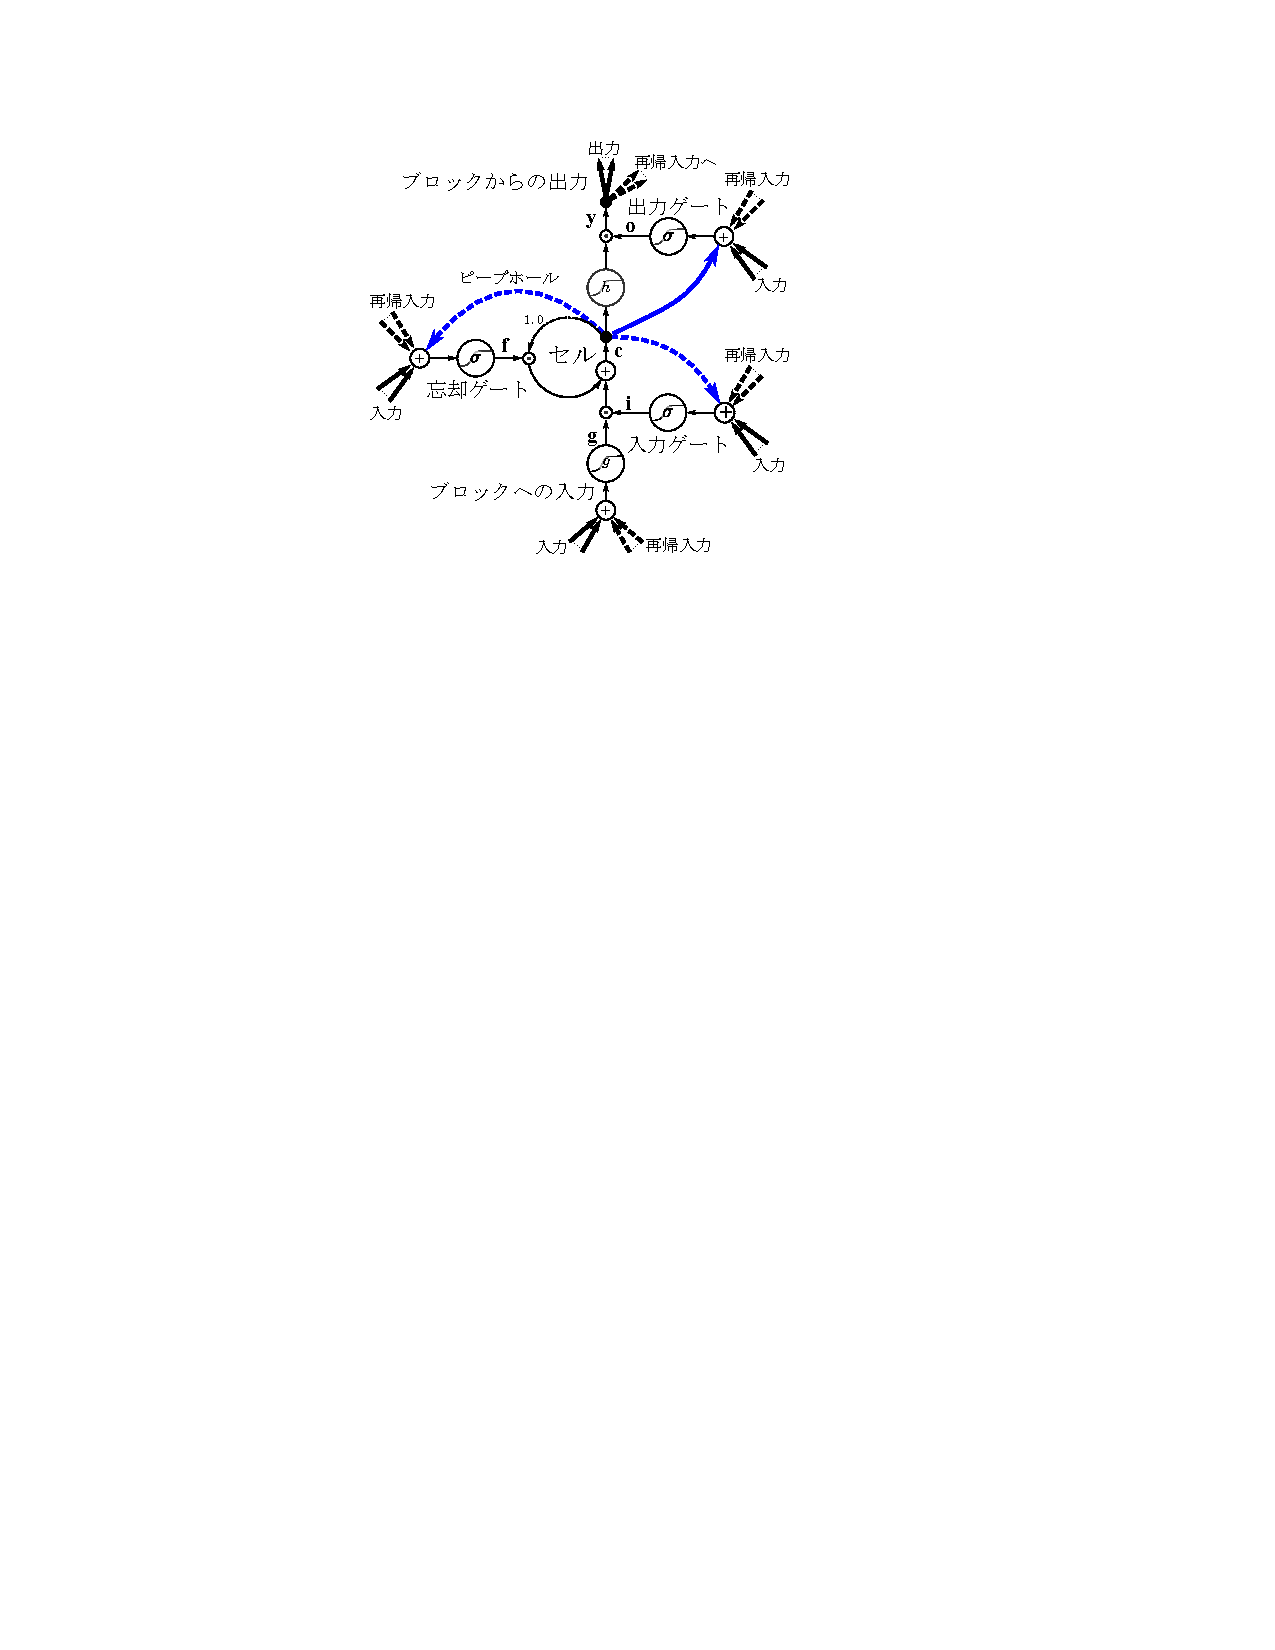
\includegraphics{2015Greff_LSTM_ja.pdf}}
\caption{\LSTM の概念図}\label{fig:LSTM}
\end{figure}
%% \begin{eqnarray}
%% i_{t}&=&\sigma\Brc{W_{xi}x_{t}+W_{hi}y_{t-1}+b_{i}},\\
%% f_{t}&=&\sigma\Brc{W_{xf}x_{t}+W_{hf}y_{t-1}+b_{f}},\\
%% o_{t}&=&\sigma\Brc{W_{xo}x_{t}+W_{ho}y_{t-1}+b_{o}},\\
%% g_{t}&=&\phi\Brc{W_{xc}x_{t}+W_{hc}y_{t-1}+b_{c}},\\
%% c_{t}&=&f_{t}\odot c_{t-1} + i_{t}\odot g_{t},\\
%% h_{t}&=&o_{t}\odot\phi\Brc{c_{t}}\label{eq:LSTM}
%% \end{eqnarray}

%% 自然言語の学習データとして,実際の人間による人工知能に関する質疑応答である
%% Web 掲示板 reddit でのやり取りを用いた。Reddit 上での質疑応答の例を図
%% \ref{fig:RedditCapture}に示す。

%% \begin{figure}[h]
%% \centering
%% \resizebox{0.4\textwidth}{!}{\rotatebox{-90}{\includegraphics{RedditCapture.pdf}}}
%% \caption{Reddit画面}\label{fig:RedditCapture}
%% \end{figure}

%% Reddit での基本的なやり取りはタイトル,質問の書き込み,回答の書き込み,となっ
%% ている。
%% 質問と回答を人間による質問($Q$)と\LSTM による回答($A$)とした。タイト
%% ルを学習者の学習状態を表す追加情報として,追加情報の影響を検証した。

入力層,単語埋込み層,\LSTM(128ユニット, 図\ref{fig:LSTM})$2$層,ソフトマッ
クス層からなる$4$層の\NN を用いた。勾配クリップを$1$に設定しドロップアウト
率$0.5$とした。BPTTの時間窓は$5$とした。

%% \subsection{追加情報を用いないLSTMによる質疑応答システム}
\subsection{一系列モデル}
\LSTM を用いた一系列モデルの概要を図\ref{fig:serial_model}に示した。
\begin{figure}[H]
\centering
\resizebox{0.3\textwidth}{!}{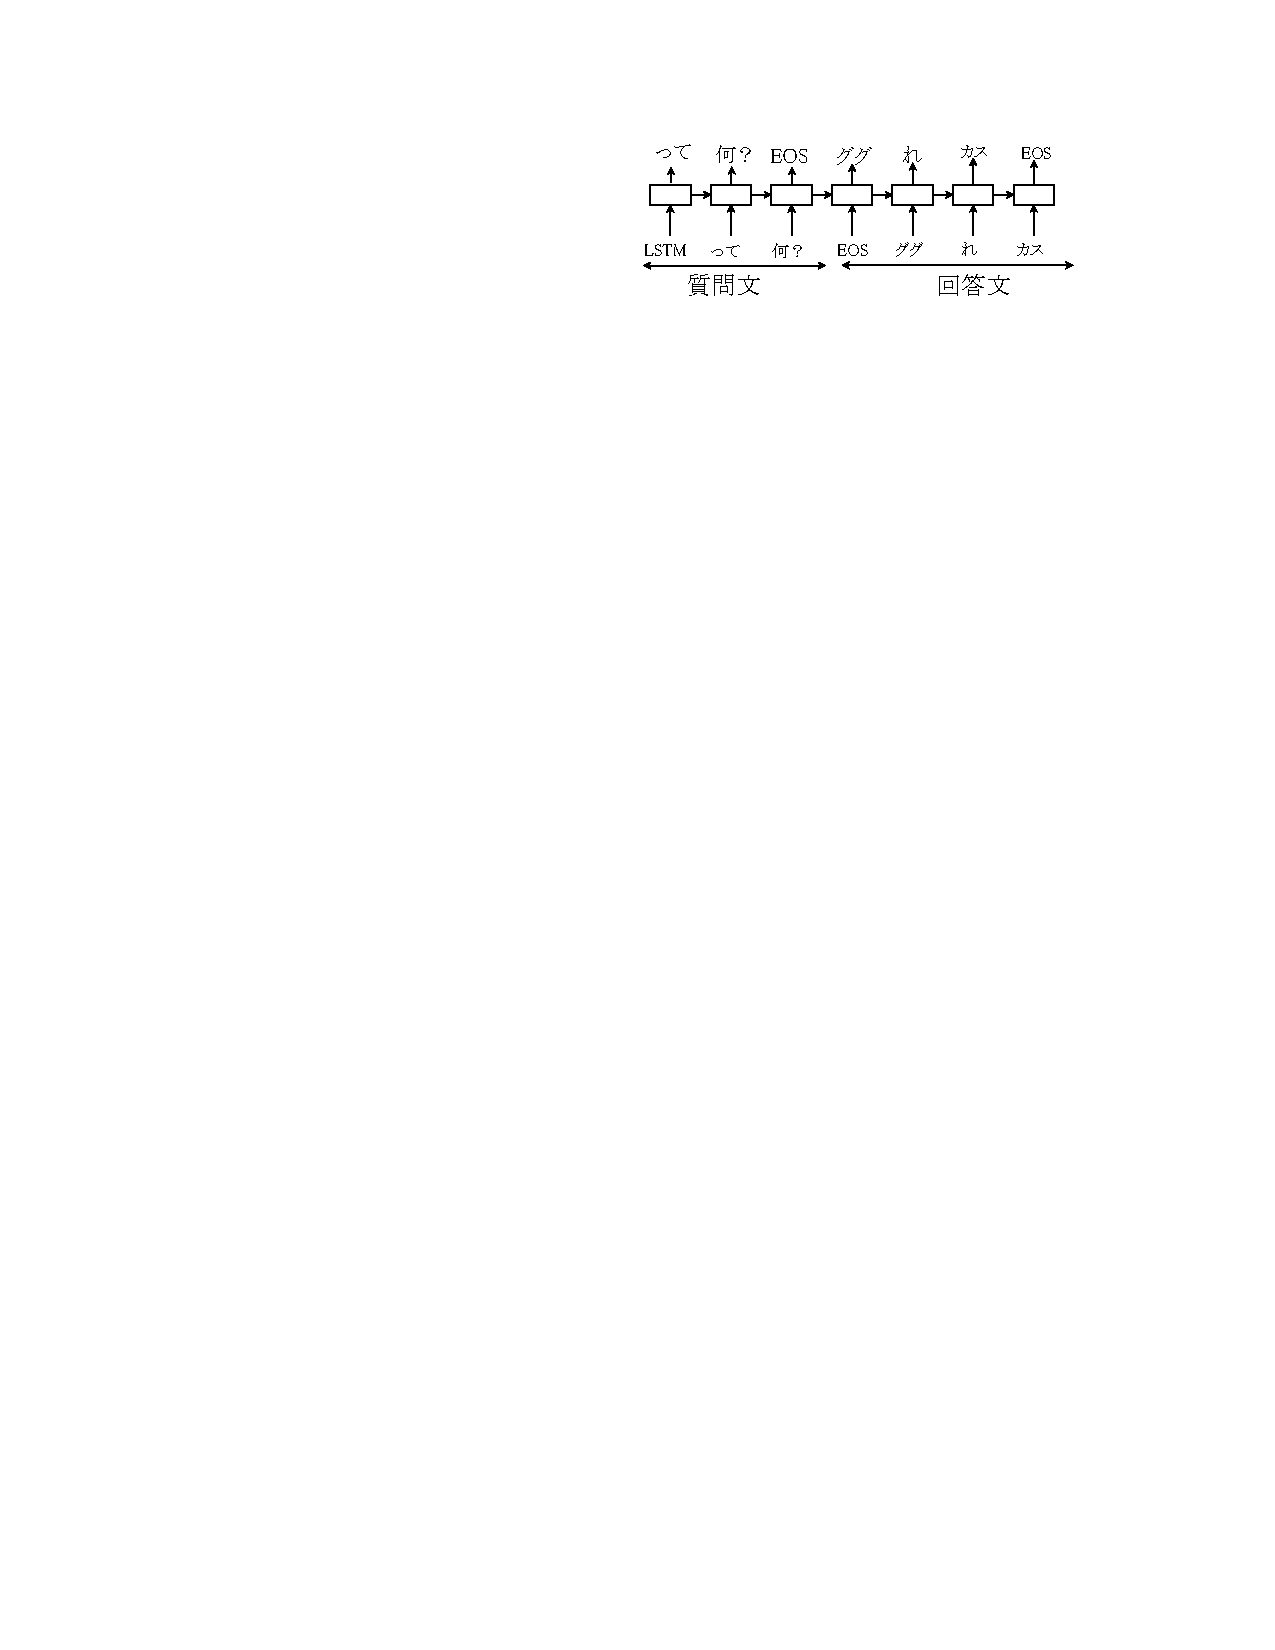
\includegraphics{dialogue_model.pdf}}
\caption{一系列モデル}\label{fig:serial_model}
\end{figure}

\subsection{対話モデル}%% 追加情報を用いた\LSTM}
%% 追加情報を加えた
%% \LSTM による質疑応答システムを実装し,学習速度,性能を測る。
\cite{2014Sutskever_Sequence_to_Sequence}による自動翻訳モデル
%% へ\LSTM を利用した
%% 研究を参考にした。
を用いた。$Q$ と $A$ とを個別の\LSTM として実装した。
%% の ユニットの概要を図\ref{fig:LSTM}に示す。
\LSTM を用いた対話モデルの概要を図\ref{fig:discours}に示した。
\begin{figure}[H]
%% \centering
  %% \resizebox{0.45\textwidth}{!}{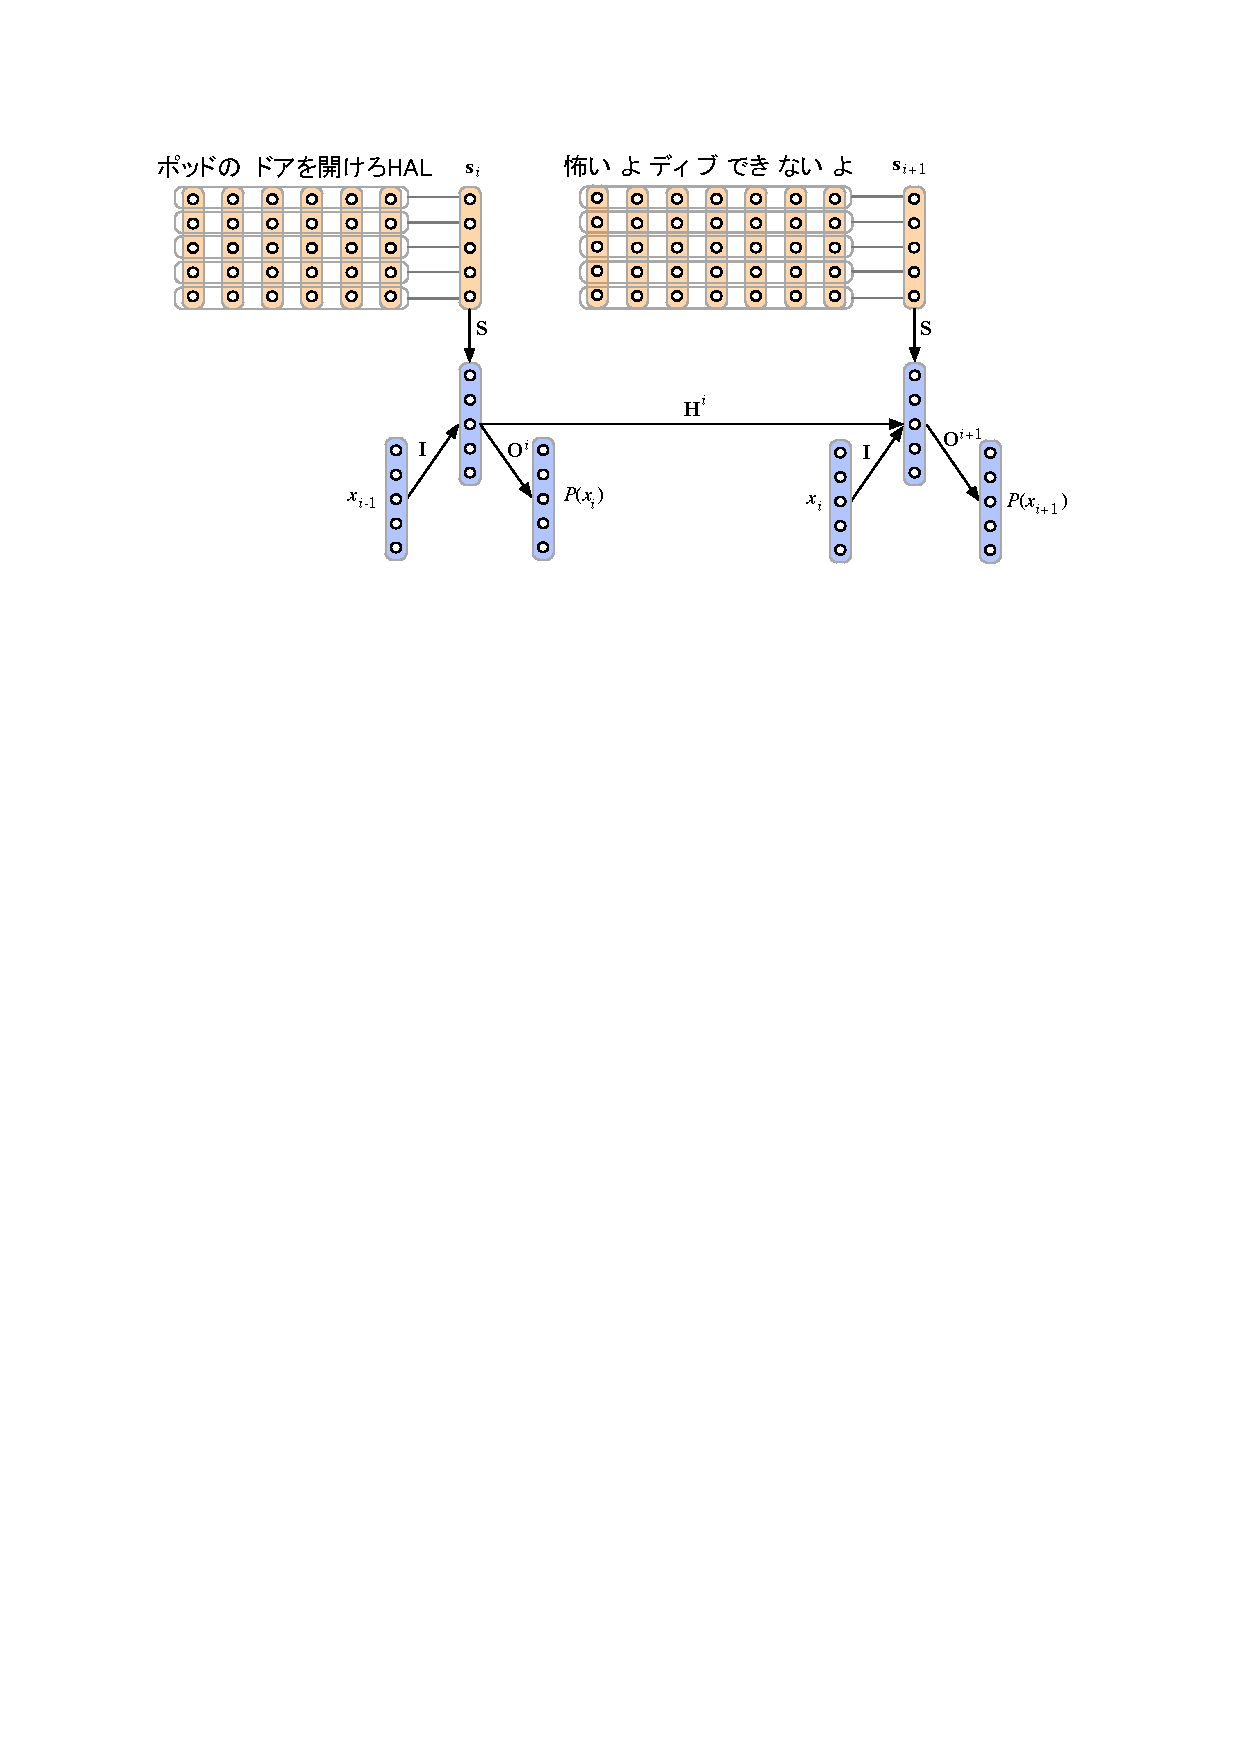
\includegraphics{2013Kalchbrenner_RCNN_Discours.pdf}}
\begin{verbatim}
<sos>  ...    <eos>    <pad>  ...   <pad>  <sos>
LSTM-->LSTM--> LSTM-->LSTM-->LSTM-->LSTM-->LSTM 
 |      |       |      |      |      |      |   
 |      |       |      |      |      |      |  
 v      v       v      v      v      v      v  
<pad>  ....   <pad>  <sos>   ...    <eos>  <pad>
LSTM-->LSTM-->LSTM--> LSTM-->LSTM-->LSTM-->LSTM
\end{verbatim}
\caption{対話モデル}\label{fig:discours}
\end{figure}
%% 追加情報を用いない質疑応答システムとしては,
$Q$ を単語ごとに入力し,その間の出力としては埋草トークン$<$PAD$>$を出力とする。
$Q$ 終了時に $Q$ 終了と示すトークン $<$EOQ$>$を入力し,$A$の先頭の単語を出
力として回答文の予測学習を行った。

\subsection{実験}
\subsubsection{データ}

Web 掲示板 \url{https://www.reddit.com/r/MLQuesitons} スレッドをスクレイピ
ングしてデータを用いた。スレッドのタイトルと本文とを質問文と見なし,回答の
ついているスレッドのみをデータとして用いた。html タグを除去した後,{NLTK}を
用いてトークン化した。一つの質問分に対して,複数の回答があるスレッドについ
ては,その都度質問文を繰り返して$\Brc{Q,A}$対を作成した。Reddit という掲示
板の性質上データセットには``{\tt :-p}'' や ``{\tt WTF}'' などの特殊な文字列
が存在した。加えて URL のみが記述された回答文も存在した。URL は {\tt
 ax{X}iv}などの論文を示しており,意味があると考えられる。しかし,処理上は
低頻度語トークンとして扱った URL も存在する。データ採取の時期柄 AlphaGo の
話題を示すURL などは低頻度語トークンに分類されずに残った。これらの傾向を期
間を限定したデータ採取では,恣意的にならずに取り扱うことは困難である。参照
先の URL が有益か否かについての判断は本研究の枠組みを超えるため取り扱わない
こととした。

総スレッド数$289$ を訓練データ($45064$語),検証データ
($10492$語),テストデータ($9509$語)に分割した。出現頻度$5$以下の低頻度語を
一括して{\tt UNK}トークンとして扱った。
%%
%% Machine learning トピック,Machine learning QA トピッ
%% ク,Machine learning Classトピックから,2016年3月26日からさかのぼって1000件
%% ずつのスレッドwを取得した。取得したスレッド中に含まれるhtml タグは {NLTK}を
%% 用いることで,変換した。
%%\subsubsection{実験環境}
%% フレームワーク
%% Chainer を用いて実装した。
%% %% 背景情報を加える版は,ソースコードを書き加えたマシンスペック~~で, n 回/day

%% \subsubsection{評価方法}
%% 類似度

\section{結果と考察}
学習済のモデルに対してテストデータを用いた評価では,データ数の関係もあり正
解データとの TD/IDF $\cos$ 類似度はそれ程高くなかった。一系列情報モデルは
$\Brc{Q,A}$対についての完全な情報を学習することを意味するので通常は有利に働
いた。一方対話モデルは$Q$の発話を受けて,$A$の系列を学習することから学習基
準に達するまでの繰り返し回数が多い傾向が見られた。ただし,TD/IDF $\cos$ 類
似度による指標では学習中の結果では一系列情報モデル $0.041$ に対して対話モデル $0.079$
となっており,有意な差異は認められなかった。

%% \section{考察}
%% 人間の講師を代替するものとして\NN での自然言語処理による学習システムを考
%% える。
%% 先行研究からは,十分なデータと適切な設定があれば,人間によるチューニングを
%% 必要としないと考えらえる。
%% 利点が報告されている。
本研究の結果は,一系列情報モデルと対話モデルとの差異が認められなかったこと
から,部分情報からの系列再生能力を用いることである程度の質疑応答システムの
開発への可能性を示すものと考えられる。
%%
%% 計算機性能の向上により適用範囲が広がり,特に注目される人工知能技術である。
%% 十分なデータと適切な設定があれば,人間によるチューニングを必要としない。将
%% 来的にあらゆる対象,分野の教育を可能にできるはず自然言語処理の分野において,
%% すでに
%% 様々な応用がされている画像からのタグ付け~\cite{2014Vinyals_Bengio_Show_and_Tell,2015Karpathy_FeiFei_caption},自動翻訳~\cite{2014Sutskever_Sequence_to_Sequence,2014Bahdanau_NMT},質疑応答~\cite{2013Kalchbrenner_EMNLP,2015Wen_EMNLP,2015Lowe}など
%% を
{QA} システム,ひいては
%の繰り返しによる
%% 教育を想定する
教育システム構築においては,学習者の理解度に合わせた適応と
低頻度語であっても有益な情報をいかに処理するかとの問題が指摘できる。
%% \NN に背景情報を入力したときの効果は,適用する問題によって意見が分
%% かれている
今後は,質問者の知識状態の推定から,回答方法の示唆など柔軟な対応を可能とする
システムの構築が望まれる。
%% \NN,とりわけ\RNN やその応用である\LSTM~\cite{1997LSTM}は文章理解,
%% 自然言語処理に用いられている。現在では応答システム~\cite{2013Kalchbrenner_EMNLP,2015Wen_EMNLP,2015Lowe}にも用いられる。\LSTM の処理能力を用いて,%%「
%% 人の教育に適応できる応答プログラム%%」
%% という
%% % 新しい
%% 可能性を模索した。
%% %% さて,
%% 教育
%% %% という
%% 場面においては質問者の理解度に応じて
%% 回答者が回答の難易度を変更する場面が求められる。%% が,
%% ここで質問者の理解というのは以前の文章を踏まえた文脈と言い換えることができる。

%% \NN において過去の時間を経て作り上げられた文脈を学習し反映することは長らくの課題であった。
%% %% add by Shin Asakawa <asakawa@ieee.org>
%% 近年では\LSTM を用いた英仏自動翻訳システム~\cite{2014Sutskever_Sequence_to_Sequence,2014Bahdanau_NMT}が提案されている。
%% %% が,
%% 過去のデータを次の中間層に直接取り込ませる手法では,% ,
%% かえって精度が低くなるという研究がなされている~\cite{2015Karpathy_Visualizing_RNN}。
%% 一方で\LSTM-RCNN を用いた画像%%の文章化
%% 脚注付け%%というタスク
%% 課題%%において
%% では\LSTM 中間層に\RCNN~\cite{2014Girshick_R-CNN,2015Girshick_FastRCNN}のデータを送ることでより性能が向上するとの論文もある
%% ~\cite{2015Karpathy_Visualizing_RNN}。%存在している。
%% %% 私たちは,
%% 我々は
%% %%「
%% 人工知能の知識習得を可能とする\LSTM による質疑応答システムの構築を目指し,
%% % ており,
%% 文章の構造理解と意味内容の学習を\LSTM を経て機械に学習させる
%% ことを %% 期待している」。
%% 目指した
%% %% (タイトル部分の挿入)そこで
%% 今回は\LSTM % の
%% モデルに文脈を新たに取り込ませる方法と,既存の\LSTM との精度の比較について比較した%%い
%% 。

%% Long Short-Term Memory (LSTM)\cite{1997LSTM}, have recently emerged as an
%% effective model in a wide variety of applications that involve sequential
%% data. These include language modeling~\cite{2010Mikolov}, handwriting
%% recognition and generation
%% ~\cite{2013Graves_handwriting,2013Graves,2012Graves}, machine translation
%% ~\cite{2014Sutskever_Sequence_to_Sequence,2014Bahdanau_NMT},
%% speech recognition~\cite{2013Graves}, video analysis~\cite{2015Donahue}
%% and image captioning
%% ~\cite{2014Vinyals_Bengio_Show_and_Tell,2015Karpathy_FeiFei_caption}.

%% A few recent ablation studies analyzed the effects on performance as
%% various gates and connections are removed Greff et
%% al~\cite{2015LSTM_SpaceOdessy}; Chung et
%% al.~\cite{2014Chung_GRU_NIPS}. However, while this analysis illuminates the
%% performance-critical pieces of the architecture, it is still limited to
%% examining the effects only on the global level of the final test set
%% perplexity alone. Similarly, an often cited advantage of the \LSTM
%% architecture is that it can store and retrieve information over long time
%% scales using its gating mechanisms, and this ability has been carefully
%% studied in toy settings Hochreiter \& Schmidhuber~\cite{1997LSTM}. However,
%% it is not immediately clear that similar mechanisms can be effectively
%% discovered and utilized by these networks in real-world data, and with the
%% common use of simple stochastic gradient descent and truncated
%% backpropagation through time.

%% \section{Overview of \LSTM}

%% As depicted at Fig. \ref{fig:LSTM}, \LSTM can be described as the input
%% signals $\mb{x}_t$ at time $t$, the output signals $\mb{o}_t$, the forget
%% gate $\mb{f}_t$, and the output signal $\mb{y}_t$, the memory cell
%% $\mb{c}_t$, then we can get the following:
%% \begin{eqnarray}
%% i_{t}&=&\sigma\Brc{W_{xi}x_{t}+W_{hi}y_{t-1}+b_{i}},\\
%% f_{t}&=&\sigma\Brc{W_{xf}x_{t}+W_{hf}y_{t-1}+b_{f}},\\
%% o_{t}&=&\sigma\Brc{W_{xo}x_{t}+W_{ho}y_{t-1}+b_{o}},\\
%% g_{t}&=&\phi\Brc{W_{xc}x_{t}+W_{hc}y_{t-1}+b_{c}},\\
%% c_{t}&=&f_{t}\odot c_{t-1} + i_{t}\odot g_{t},\\
%% h_{t}&=&o_{t}\odot\phi\Brc{c_{t}}\label{eq:LSTM}
%% \end{eqnarray}

%% \section{Model proposed}
%% We can summarized

%% \section{Experiment}
%% \subsection{Data sets}
%% Karpathy and Fei-Fei Li~\cite{2015Karpathy_Visualizing_RNN} chose to use Leo
%% Tolstoy's War and Peace (WP) novel, which consists of 3,258,246 characters
%% of almost entirely English text with minimal markup, and at the other end
%% of the spectrum the source code of the Linux Kernel (LK).  They shuffled
%% all header and source files randomly and concatenated them into a single
%% file to form the 6,206,996 character long dataset. They split the data into
%% train/val/test splits as 80/10/10 for WP and 90/5/5 for LK. Therefore,
%% there were approximately 300,000 characters in the validation/test splits
%% in each case. The total number of characters in the vocabulary is 87 for WP
%% and 101 for LK.

%% \subsection{Comparing Recurrent Networks}
%% Karpathy and Li first trained several \RNN models to support further
%% analysis and to compare their performance in a controlled setting. In
%% particular, they trained models in the cross product of type
%% (\LSTM/\RNN/\GRU), number of layers (1/2/3), number of parameters (4
%% settings), and both datasets (WP/KL). For a 1-layer \LSTM they used hidden
%% size vectors of 64,128,256, and 512 cells, which with their character
%% vocabulary sizes translates to approximately $50$~K, $130$~K, $400$~K, and
%% $1.3$~M parameters respectively. The sizes of hidden layers of the other
%% models were carefully chosen so that the total number of parameters in each
%% case is as close as possible to these $4$ settings.

%% \begin{figure}[H]
%% \centering
%% \resizebox{0.4\textwidth}{!}{\includegraphics{2015Karpathy_Fig1_1.pdf}}
%% \caption{hoge}
%% \end{figure}

\bibliography{asakawa}
\bibliographystyle{jsai}

\end{document}


\section{全般的事項}

\subsection{ファイル形式・サイズ}

Adobe(R) PDF (Portable Document Format) 形式 のファイルを提出してく
ださい.その他の形式での提出は受け付けませんので,ご注意ください.ファ
イルサイズはファイル受付システムの制限がありますので,3MB 以下にしてく
ださい.また,ファイル名の拡張子は .pdf にしてください.

\subsection{ヘッダー部分}

\bf \textcolor{red}{今大会から講演番号およびヘッダの会議名は,原稿提出後に運営側で挿入しますので,著者が作成する原稿には記入しないでください.}

\subsection{原稿枚数}

下記指定フォーマットでA4用紙2ページです.希望によりさらに2ページまで無
料で追加できます.


\section{\LaTeX{}原稿のスタイル}

論文のスタイルを統一するために,原稿はできるだけ以下のスタイルファイル
を使ってください.基本的には2000年度までの全国大会論文集用に配布されて
いた原稿用紙と同じ形に仕上がるようになっています.スタイルファイル自体
は昨年度用のものと同一です.

スタイルファイルは以下のように指定してください.

ASCII版\LaTeX{}2.09なら
\begin{verbatim}
\documentstyle[twocolumn,jsaiac]{jarticle}
\end{verbatim}

NTT版\LaTeX{}2.09なら
\begin{verbatim}
\documentstyle[twocolumn,jsaiac]{j-article}
\end{verbatim}

ASCII版\LaTeXe{}なら
\begin{verbatim}
\documentclass[twocolumn]{jarticle}
\usepackage{jsaiac}
\end{verbatim}

欧文使用の\LaTeX{}2.09なら
\begin{verbatim}
\documentstyle[twocolumn,jsaiac]{article}
\end{verbatim}

欧文使用の\LaTeXe{}なら
\begin{verbatim}
\documentclass[twocolumn]{article}
\usepackage{jsaiac}
\end{verbatim}

\Style{}は以上のように,標準で配布されるパッケージである
jarticle.sty,j-article.sty,jarticle.cls
(欧文論文の場合はarticle.sty,article.cls)を主のスタイルファイルとして,
それにオプションという形で使うように設定されています.
\Style{}はタイトル部分,文字組の調整,一部脚注の
調整以外は行っていませんが,
共通版にする関係から,オプションのtwocolumnの指定が必須です.
以上のことから,
\Style{}を使う場合は,上記の指定方法を必ず守るようお願いいたします.

\Style{}は以上の3つの\LaTeX{}のバージョンに対応しています.
NTT版の\LaTeXe{}は動作確認を行っていません.

\subsection{\Style{}を使うことで指定が不要なもの}

\Style{}を使えば,次の指定は必要ありません.

\begin{itemize}
\item ページ番号の書式
\item マージン等の位置
\item 用紙(A4)用紙
\item 本文(2段組)
\end{itemize}

\subsection{\Style{}を使うことで指定が必要なもの}

\def\Label{\vskip.5\baselineskip\noindent$\circ$\hskip3pt{}}

\Label タイトル領域: \Style{}の書き方のきまりは次のようになります.
\begin{itemize}
\item タイトル: 
\begin{verbatim}
\title{
   \jtitle{和文タイトル}
   \etitle{欧文タイトル}
}
\end{verbatim}
なお,欧文論文の場合は,単に
\begin{verbatim}
\title{欧文タイトル}
\end{verbatim}
としてください.
\item 筆者名(同一所属の場合): 

\begin{verbatim}
\author{%
   \jname{筆者氏名}
   \ename{Given-name Surname}
\and
   \jname{筆者氏名}
   \ename{Given-name Surname}
\and
   Given-name Surname
}
\end{verbatim}

なお,欧文論文の場合は,単に
\begin{verbatim}
\author{%
   Given-name Surname
\and
   Given-name Surname
}
\end{verbatim}
としてください.\verb|\jname{ }|や\verb|\ename{ }| は指定しません.
\item 筆者名(所属が異なる場合): 
\begin{verbatim}
\author{%
   \jname{第1筆者氏名\first{}}
   \ename{Given-name Surname}
\and
   \jname{第2筆者氏名\second{}}
   \ename{Given-name Surname}
\and
   Given-name Surname\third{}
}
\end{verbatim}
所属が異なる場合,違いを識別するため,
\begin{verbatim}
\first   \second    \third .... 
\end{verbatim}
の指定を加えてください.これは
同一の所属は同一のコマンドを与えます.
さらに所属の方にも,該当する \verb|\first|,\linebreak
\verb|\second|,
\verb|\third|$\cdots$ の指定を加えますが,その順序は自由です.
具体的な出力は,\verb|\first| と指定すると,``$^{\ast 1}$''が
筆者名の右上(所属は左上)に表示されます.
これは単純なコマンドです.全部で9つ用意してあります.
以下がその内訳です.
\begin{verbatim}
\def\first{\hbox{$\m@th^{\ast 1}$\hss}}
\def\second{\hbox{$\m@th^{\ast 2}$\hss}}
\def\third{\hbox{$\m@th^{\ast 3}$\hss}}
\def\fourth{\hbox{$\m@th^{\ast 4}$\hss}}
\def\fifth{\hbox{$\m@th^{\ast 5}$\hss}}
\def\sixth{\hbox{$\m@th^{\ast 6}$\hss}}
\def\seventh{\hbox{$\m@th^{\ast 7}$\hss}}
\def\eighth{\hbox{$\m@th^{\ast 8}$\hss}}
\def\ninth{\hbox{$\m@th^{\ast 9}$\hss}}
\end{verbatim}

\item 所属: \verb|\jname{ }|や\verb|\ename{ }| の指定は筆者名の場合と
同じです.次のように指定します.
\begin{verbatim}
\affiliate{
   \jname{\first{}所属和文1}
   \ename{Affiliation #1 in English}
\and
   \jname{\second{}所属和文2}
   \ename{Affiliation #2 in English}
\and
   \third{}Affiliation #3 in English
}
\end{verbatim}
なお,欧文論文の場合は,単に
\begin{verbatim}
\affiliate{
   \first{}Affiliation #1 in English
\and
   \second{}Affiliation #2 in English
\and
   \third{}Affiliation #3 in English
}
\end{verbatim}
とします.\verb|\jname{ }|や\verb|\ename{ }| は指定しません.
ただし,和欧文とも所属が同一の場合は,\verb|\first| の指定は不要です。

\item 連絡先: 代表者の氏名,所属,所在地,電話番号,Fax番号, 
e-mail アドレスなどをお書き下さい.
\begin{verbatim}
\jaddress{氏名,所属,住所,電話番号,Fax番号,電子メールアドレスなど}
\end{verbatim}
とすれば,脚注の位置に``連絡先:~''という形で出力されます.
なお,欧文論文の場合は,
\begin{verbatim}
\address{name, affiliation, address, 
telephone number, Fax number, 
e-mail address}
\end{verbatim}
とすれば,脚注の位置に``Contact:~''という形で出力されます.
\end{itemize}

\Label その他
\begin{itemize}
\item 脚注: 脚注は,下にある例のように\footnote{この例が脚注です.}
通常の\LaTeX{}\linebreak
(\cite{latexブック})の
書き方である\verb|\footnote{  }| を使って書きます.
\item 参考文献: j(-)article.cls(sty)(欧文論文の場合は
article.sty(cls))が用意しているものを使うことになります.
著者名,文献名,ジャーナル(出版社),発行年など,イニシャル,
略語のスタイル,記載順などは論文誌の規則に従ってください.
\JBibTeX{}を使う場合は論文誌用の\LaTeX{}スタイルファイルと
同時に配布されている``jsai.bst''を使うことをお勧めします.
参照ラベルの \verb|\cite{ }| も使えます.
最後の部分に参考文献のサンプルが添付してあります.
\item 他のコマンド 通常の\LaTeX{}の組版と変わりありません.
j(-)article.cls{sty}(欧文論文の場合はarticle.sty(cls))で
扱えるものはすべて使うことができます.
\end{itemize}

%% \begin{thebibliography}{99}
%% \bibitem[Knuth 84]{texbook}
%%  Knuth,~D.~E.: The \TeX{}book, Addison-Wesley (1984),
%%   (邦訳~: \TeX{}ブック, 斎藤 信男 監修, 鷺谷 好輝 訳,
%%   アスキー出版局 (1992)).
%% \bibitem[Lamport 86]{latexブック}
%% Leslie,~L: \LaTeX{}: {A} Document Preparation System (Updated for
%%   \LaTeX{}2$\varepsilon$), Addison-Wesley, 2nd edition (1998)
%%   (邦訳~: 文書処理システム \LaTeX{}2$\varepsilon$,
%%   阿瀬 はる美 訳, ピアソン・エデュケーション, (1999)).
%% \end{thebibliography}
%% %%




%% What is Karma on Reddit:
%% Reddit karma is one of the gamification techniques used to engage users
%% on reddit. It's pretty similar to Quora credits - You get more karma
%% when your posts/comments get upvoted, and lose some when they get
%% downvoted.
%%
%% https://www.quora.com/What-is-Reddit-karma-and-how-do-people-benefit-from-having-more-Reddit-karma
%% What is Reddit karma and how do people benefit from having more Reddit
%% karma?
%%
%% Eeshan Malhotra

%% Reddit karma is one of the gamification techniques used to engage users
%% on reddit. It's pretty similar to Quora credits - You get more karma
%% when your posts/comments get upvoted, and lose some when they get
%% downvoted. There are two key differences I can think of:
%%
%% Reddit karma can not be 'redeemed' for anything, even on the
%% website. Quora credits can be used to ask questions, for A2As, and for
%% promoting content (Although, for a number of users, the credits they
%% have accumulated are enough to be able to do all of that without really
%% caring for their credit reserve)
%%
%% Reddit karma is displayed publicly. This means that everyone who wants
%% to know how much karma a user has accumulated, can readily find this
%% out. So redditors take pride in their karma (kind of like having a high
%% score at an arcade), and karma is often associated with respect on
%% reddit.
%%
%% So essentially, both Quora credits and Reddit karma take some aspects of
%% real world currency. While credits focus more on the aspect of
%% 'purchasing' stuff with money, karma has more to do with flaunting your
%% riches.

%% https://www.reddit.com/wiki/faq
%% Frequently Asked Questions

%% Basics
%%
%% What is reddit?
%%
%% reddit is a source for what's new and popular on the web.
%%
%% Users like you provide all of the content and decide, through voting,
%% what's good and what's junk.
%%
%% Links that receive community approval bubble up towards #1, so the front
%% page is constantly in motion and (hopefully) filled with fresh,
%% interesting links.
%%
%% What does the name "reddit" mean?
%%
%% It's (sort of) a play on words -- i.e., "I read it on reddit." Also,
%% there are some unintentional but interesting Latin meanings to the word
%% "reddit". Details \link(here).

%% What is that alien / bug thing?
%%
%% That adorable and informative creature is Snoo, the mascot for the
%% reddit community. It is also a registered trademark owned by reddit. You
%% can visit redditalien.com for an archive of its past adventures.

%% Can anyone submit a link?

%% Yes — all you need is an account! However, there is a cap on the
%% posting rate to prevent spamming. This restriction is the same for both
%% reddit gold members and non-gold members.

%% How is a submission's score determined?

%% A submission's score is simply the number of upvotes minus the number of
%% downvotes. If five users like the submission and three users don't it
%% will have a score of 2. Please note that the vote numbers are not "real"
%% numbers, they have been "fuzzed" to prevent spam bots etc. So taking the
%% above example, if five users upvoted the submission, and three users
%% downvote it, the upvote/downvote numbers may say 23 upvotes and 21
%% downvotes, or 12 upvotes, and 10 downvotes. The points score is correct,
%% but the vote totals are "fuzzed".

%% Why does a dot sometimes show up where the score should be?

%% For the first few hours after a submission is created, the score is not
%% displayed. This is intended to mitigate the bandwagon effect.

%% I made a mistake in my submission title, how can I edit it?

%% Submission titles cannot be edited. However, you can simply delete it
%% and resubmit it. The sooner you do this, the less likely you will lose
%% any votes or comments.

%% What is that number next to usernames? And what is karma?

%% The number next to a username is called that user's "karma." It reflects
%% how much good the user has done for the reddit community. The best way
%% to gain karma is to submit links that other people like and vote for,
%% though you won't get karma for self posts.

%% Why should I try to accumulate karma?

%% Why should you try to score points in a video game? Why should your
%% favorite sports team try to win the championship?

%% Or, to look at things from a less competitive and more altruistic
%% perspective, read what philosophers have said about the matter --
%% namely, don't set out to accumulate karma; just set out to be a good
%% person, and let your karma simply be a reminder of your legacy. Note:
%% reddit makes no guarantees about attaining Nirvana.

%% Update: A redditor named jumpercable tried to redeem his karma. See how
%% it went (your mileage may vary).

%% What can I do to get my submissions noticed?

%% Remember that adage about not judging a book by its cover? No one
%% actually follows it. So choose your title carefully — make it useful,
%% provide context, and be descriptive. Be careful though, if you're too
%% aggressive it could backfire. Phrases like, "Vote this up to spread the
%% word!" or "AMAZING!" tend to annoy most redditors, who will make sure
%% your post doesn't see the light of day.

%% Why don't my submissions show up on the New page?

%% reddit has a spam filter designed to detect spam posts and automatically
%% remove them. However, legitimate posts are often caught by the
%% filter. If a few minutes go by and your post isn't showing up on the new
%% page of the community where you posted, it has probably been caught by
%% the filter. This is most likely to occur if you are posting to a
%% community that you have not participated in before. Each community has
%% an independent filter, for example /r/help's filter doesn't talk to
%% /r/pic's filter. In order to remove your post from the filter you need
%% to message the moderators (this link can be found in the sidebar on the
%% right-hand in that community, you can also manually compose a message to
%% #communityname) and ask them to check the filter for you. Eventually the
%% filter will "learn" that your posts don't need to be removed.

%% Is reddit available in languages other than English?

%% Yes! In the upper-right corner of the page, there should be a link that
%% says, "English". Click it and you'll get a popup where you can change to
%% another language.

%% I want to change my username. Do I have to start a new account?

%% Yes. Once a user account is created, the username cannot be edited. You
%% can create a new user profile but cannot migrate karma, comment karma or
%% trophies to the new username.

%% Will you remove something defamatory about me or "my friend" from
%% reddit?

%% In light of the protections afforded to online hosts of third party
%% content, such as reddit, we rarely remove such material, but we reserve
%% the right to do so for legal or other reasons.

%% Please note that reddit does not remove posts for containing insults or
%% negative commentary, but leaves such decisions to the moderators of
%% particular communities. Those moderators are not employees of or
%% retained by reddit‚ they are the persons who initiated the particular
%% community and their appointees. While posts that contain such content
%% can be distasteful, reddit is not in a position to arbitrate
%% disputes. Posts should be consistent with the rules of the community to
%% which they are posted.

%% The best way to deal with incorrect information on the Internet is to
%% post the correct information next to it. The reddit community is usually
%% very supportive of such a response, and will likely vote to give the
%% correction greater prominence than the original post. Redditors love a
%% good counterpoint.

%% Is posting personal information ok?

%% NO. reddit is a pretty open and free speech place, but it is not ok to
%% post someone's personal information, or post links to personal
%% information. This includes links to public Facebook pages and
%% screenshots of Facebook pages with the names still legible. We all get
%% outraged by the ignorant things people say and do online, but witch
%% hunts and vigilantism hurt innocent people and certain individual
%% information, including personal info found online is often
%% false. Posting personal information will get you banned. Posting
%% professional links to contact a congressman or the CEO of some company
%% is probably fine, but don't post anything inviting harassment, don't
%% harass, and don't cheer on or vote up obvious vigilantism.

%% Is posting political campaign information ok?

%% Yes. reddit does not discriminate among candidates or differing
%% political viewpoints in any way, nor does it discriminate between
%% political and non-political topics. reddit's terms of service require
%% all users not to violate any law, statute or regulation in the course of
%% their use. reddit provides its basic service to all users without charge
%% and its provision of basic services for free is not a contribution to
%% any candidate, political committee, or political party committee. reddit
%% does not control links to political sites, does not endorse them, and is
%% not responsible for any aspects of those sites.

%% Which staff member should I write to if I have a problem or question?

%% Send a message to /r/reddit.com

%% I want to make something with the reddit alien on it. Whom do I contact?

%% We have a whole page on licensing.

%% What do all of these acronyms mean?

%% Well there are a lot of acronyms in use on reddit, so this is just a
%% list of some of the main ones you'll see.

%% AFAIK means "As far as I know"
%% AMA means "Ask me anything"
%% CMV means "Change my view"
%% DAE means "Does anybody else" or "Does anyone else"
%% ELI5 means "Explain like I'm 5 (years old)"
%% FTFY means "Fixed that for you"
%% IAMA means "I am a"
%% IANAD means "I am not a doctor"
%% IANAL means "I am not a lawyer"
%% IIRC means "If I recall correctly"
%% IMO/IMHO means "In my opinion" and "In my humble/honest opinion", respectively
%% ITT means "In this thread"
%% MRW/MFW means "My reaction when" and "My face when", respectively
%% NSFL means "Not safe for life" (gory or gross content)
%% NSFW means "Not safe for work" (sexual content)
%% OP means "Original poster" (the person who started the thread)
%% [Serious] means "Serious responses only" (commonly used in /r/askreddit and other subreddits now)
%% PSA means "Public service announcement"
%% TIL means "Today I learned"
%% TL;DR means "Too long; Didn't read"
%% YSK means "You should know"
%% Commenting

%% Is there a reference guide for the reddit comment syntax?

%% Yes — the commenting help page explains all the details, pitfalls, and
%% workarounds.

%% What does it mean when an asterisk appears next to a comment?

%% This just means that the commenter has edited it. (On reddit, you can go
%% back and edit your comments in order to fix mistakes, add new
%% information, or be annoying.)

%% How is a comment's score determined?

%% According to the same principles as a submission's score.

%% A comment's score is simply the number of upvotes minus the number of
%% downvotes. If five users like the comment and three users don't it will
%% have a score of 2. Please note that the vote numbers are not "real"
%% numbers, they have been "fuzzed" to prevent spam bots etc. So taking the
%% above example, if five users upvoted the comment, and three users
%% downvote it, the upvote/downvote numbers may say 23 upvotes and 21
%% downvotes, or 12 upvotes, and 10 downvotes. The points score is correct,
%% but the vote totals are "fuzzed".

%% Individual subreddits

%% What are subreddits?

%% reddit is made up of thousands of sub-communities, each focused on a
%% specific topic. There's a subreddit for science, a subreddit for music,
%% and probably a subreddit for your nearest city. By default, new users
%% are subscribed to a selection of the most popular ones, but you'll get a
%% lot more enjoyment out of the site if you take the time to subscribe to
%% ones that appeal to you. After doing so, the front page will change to
%% show a customized listing tailored to your interests.

%% How can I find and subscribe to subreddits?

%% There are several ways. If you already know what you're looking for, or
%% simply want to browse the list in order of popularity, the reddit search
%% page will be most direct. There are also a number of external,
%% unofficial but authorized sites that provide different interfaces,
%% e.g. metareddit.com, subredditfinder.com, subreddits.org. To see new
%% subreddits as they're created, subscribe to the subreddit
%% /r/newreddits. Finally, to find a random subreddit, visit /r/random.

%% You can browse a subreddit before subscribing to it, and if you decide
%% to join, there's a "subscribe" link on the right side of every page. If
%% you're already subscribed you can click "unsubscribe" to unsubscribe.

%% How many subreddits can I subscribe to?

%% You may subscribe to as many subreddits as you like! However, on any
%% given visit, your frontpage will only select up to 50 subreddits to show
%% you (100 for gold users). This selection is refreshed every 30
%% minutes. When you view the 'MY SUBREDDITS' dropdown, you are seeing only
%% the current 50 selected. The only place to see all the subreddits you
%% are subscribed to is here.

%% Do any subreddits have their own FAQs?

%% Many do. Check out /r/somesubreddit/wiki to see if your favorite has
%% one.

%% Moderators

%% What is a moderator?

%% A moderator is just a regular redditor like you except they volunteer to
%% perform a few humble duties within a particular community:

%% They configure parameters for the community, like what its description
%% should be or whether it should be considered "Over 18".  They set the
%% custom logo and styling, if any.  They can mark their own links or
%% comments as the community moderator's submission, which just adds an
%% "[M]" and turns their name green.  They can remove links and comments
%% from their community if they find them objectionable or off topic.  They
%% can ban a spammer or other abusive user from submitting to their
%% community. (This has no effect elsewhere on the site).  They can add
%% other users as moderators.  Moderators have no special powers outside of
%% the community they moderate and are not appointed by reddit.

%% Why does reddit need moderation? Can't you just let the voters decide?

%% The reason there are separate subreddits is to allow niche communities
%% to form, instead of having one monolithic overall community. These
%% communities distinguish themselves with a unique focus, look and
%% policies: what's on- and off-topic there, whether people are expected to
%% behave civilly or can feel free to be brutal, etc.

%% One issue that arises is that casual, new, or transient visitors to a
%% particular community don't always know the rules that tie it together.

%% As an example, imagine a /r/swimming and a /r/scuba. People can read
%% about one topic or the other (or subscribe to both). But since scuba
%% divers like to swim, a casual user might start submitting swimming links
%% on /r/scuba. And these stories will probably get upvoted, especially by
%% people who see the links on the reddit front page and don't look closely
%% at where they're posted. If left alone, /r/scuba will just become
%% another /r/swimming and there won't be a place to go to find an
%% uncluttered listing of scuba news.

%% The fix is for the /r/scuba moderators to remove the offtopic links, and
%% ideally to teach the submitters about the more appropriate /r/swimming
%% subreddit.

%% What if the moderators are bad?

%% In a few cases where a moderator has lost touch with their community,
%% another redditor has created a competing community and subscribers have
%% chosen to use the new reddit instead, which led to it becoming the new
%% dominant reddit.

%% If you have an issue with a moderator or the way a subreddit is being
%% run, please first try contacting that moderator to see if it's just a
%% simple misunderstanding. You may contact all of the moderators in a
%% subreddit by messaging /r/[name of subreddit] to appeal a
%% decision. Please keep in mind, however, that moderators are free to run
%% their subreddits however they so choose so long as it is not breaking
%% reddit's rules. So if it's simply an ideological issue you have or a
%% personal vendetta against a moderator, consider making a new subreddit
%% and shaping it the way you'd like rather than performing a sit-in and/or
%% witch hunt.

%% How do you get to be a moderator?

%% If you create a subreddit you will automatically become its
%% moderator. If you'd like to become a moderator of an existing subreddit,
%% ask one of the community's moderators! Many subreddits actively look for
%% volunteers, so feel free to head on over to /r/needamod and see who
%% needs help. If you find an abandoned subreddit, a final option would be
%% to check out /r/redditrequest and make a post requesting to be a
%% moderator.

%% How can I tell who moderates a given subreddit?

%% While visiting that subreddit's front page, there should be a box on the
%% right with the names of all its moderators. If you can't find it, just
%% go to http://reddit.com/r/name-of-subreddit/about/moderators directly.

%% Where can I find more information about moderation?

%% Here.
%% Spam, Cheating, and the Like

%% Is it okay to create multiple accounts?

%% Yes, you can create multiple/throwaway accounts as long as you do not do
%% so to ghost vote your own submissions.

%% Why isn't my submission / comment showing up?

%% Submissions can take a few minutes to appear on the New queue. But it's
%% also possible that a moderator deemed your post to be spam -- or the
%% automatic filtering program did. If you feel this was a mistake, try
%% sending a message to a moderator of the subreddit in question. If they
%% do not respond after a day or so, post a question in /r/help.

%% What is the "report" button?

%% The report button, shown on all links and comments, is an anonymous way
%% for the reddit community to send feedback to the moderators that
%% something is spam or otherwise violates the rules -- for example,
%% pornographic content submitted to a non-adult subreddit, or a .PDF
%% posted to /r/videos. If your reason for reporting is time-sensitive or
%% non-obvious, please leave a reply or send a message to a moderator
%% explaining your reasoning.

%% You can also report spam by submitting the offending user's overview
%% page to the /r/spam subreddit.

%% What happens when something gets reported?

%% It will be reviewed, either by a person or a program. The more people
%% who report it, the more likely some action will be taken. Reporting spam
%% is the single most important thing a user can do to help keep reddit
%% clean.

%% What constitutes vote cheating and vote manipulation?

%% Besides spam, the other big no-no is to try to manipulate voting by any
%% means: manual, mechanical, or otherwise. We're not going to post an
%% exhaustive list of forbidden tactics (lest we give people ideas), but
%% some major ones are:

%% Don't use shill or multiple accounts, voting services, or any other
%% software to increase votes for submissions Don't ask other users to vote
%% on certain posts, either on reddit itself or anywhere else (through
%% Twitter, Facebook, IM programs, IRC, etc.)  Don't be part of a "voting
%% clique" or "vote ring" A voting clique is a group of people who send
%% links to their submissions around via message, IM, or any other means,
%% with the expectation of "you guys vote for my stuff and I'll vote for
%% yours." A "vote ring" is a group of people who agree to vote on certain
%% things together, either a specific submission, a user, a domain, or
%% anything like that. Upvote each submission or content for the value of
%% the information in it, a variety of things that you think are
%% interesting and will benefit the community.

%% Cheating or attempting to manipulate voting will result in your account
%% being banned. Don't do it.

%% What constitutes spam?

%% It's a gray area, but some rules of thumb:

%% It's not strictly forbidden to submit a link to a site that you own or
%% otherwise benefit from in some way, but you should sort of consider
%% yourself on thin ice. So please pay careful attention to the rest of
%% these bullet points.  If your contribution to reddit consists mostly of
%% submitting links to a site(s) that you own or otherwise benefit from in
%% some way, and additionally if you do not participate in discussion, or
%% reply to peoples questions, regardless of how many upvotes your
%% submissions get, you are a spammer. If over 10\% of your submissions and
%% conversation are your own site/content/affiliate links, you're almost
%% certainly a spammer.  If people historically downvote your links or ones
%% similar to yours, and you feel the need to keep submitting them anyway,
%% they're probably spam.  If people historically upvote your links or ones
%% like them -- and we're talking about real people here, not sockpuppets
%% or people you asked to go vote for you -- congratulations! It may not be
%% spam! However, you still need to follow the guidelines for self
%% promotion If nobody's submitted a link like yours before, give it a
%% shot. But don't flood the new queue; submit one or two times and see
%% what happens.  To play it safe, write to the moderators of the community
%% you'd like to submit to. They'll probably appreciate the advance
%% notice. They might also set community-specific rules that supersede the
%% ones above. And that's okay -- that's the whole point of letting people
%% create their own reddit communities and define what's on topic and
%% what's spam.

%% If you're thinking of doing any self-promotion on reddit, you might want
%% to read this first.

%% Nerd Talk

%% What is reddit written in?

%% Python.

%% Seriously? I heard it was written in Lisp.

%% It was, but we rewrote it. (Here's why.)

%% So what Python framework do you use?

%% Pylons. You can see our source code if you want.

%% Anything we didn't cover?

%% If you have a question that isn't answered here, you can get
%% near-instant assistance by reading the /r/help FAQ or posting on the
%% /r/help reddit. We also have press information available, and a page for
%% those looking to advertise on reddit. If you're new to reddit and want
%% some more information on interesting subreddits, confusing acronyms and
%% so on, try this post..
